\section{Text Class Reference}
\label{classText}\index{Text@{Text}}
{\tt \#include $<$text.h$>$}

Inheritance diagram for Text::\begin{figure}[H]
\begin{center}
\leavevmode
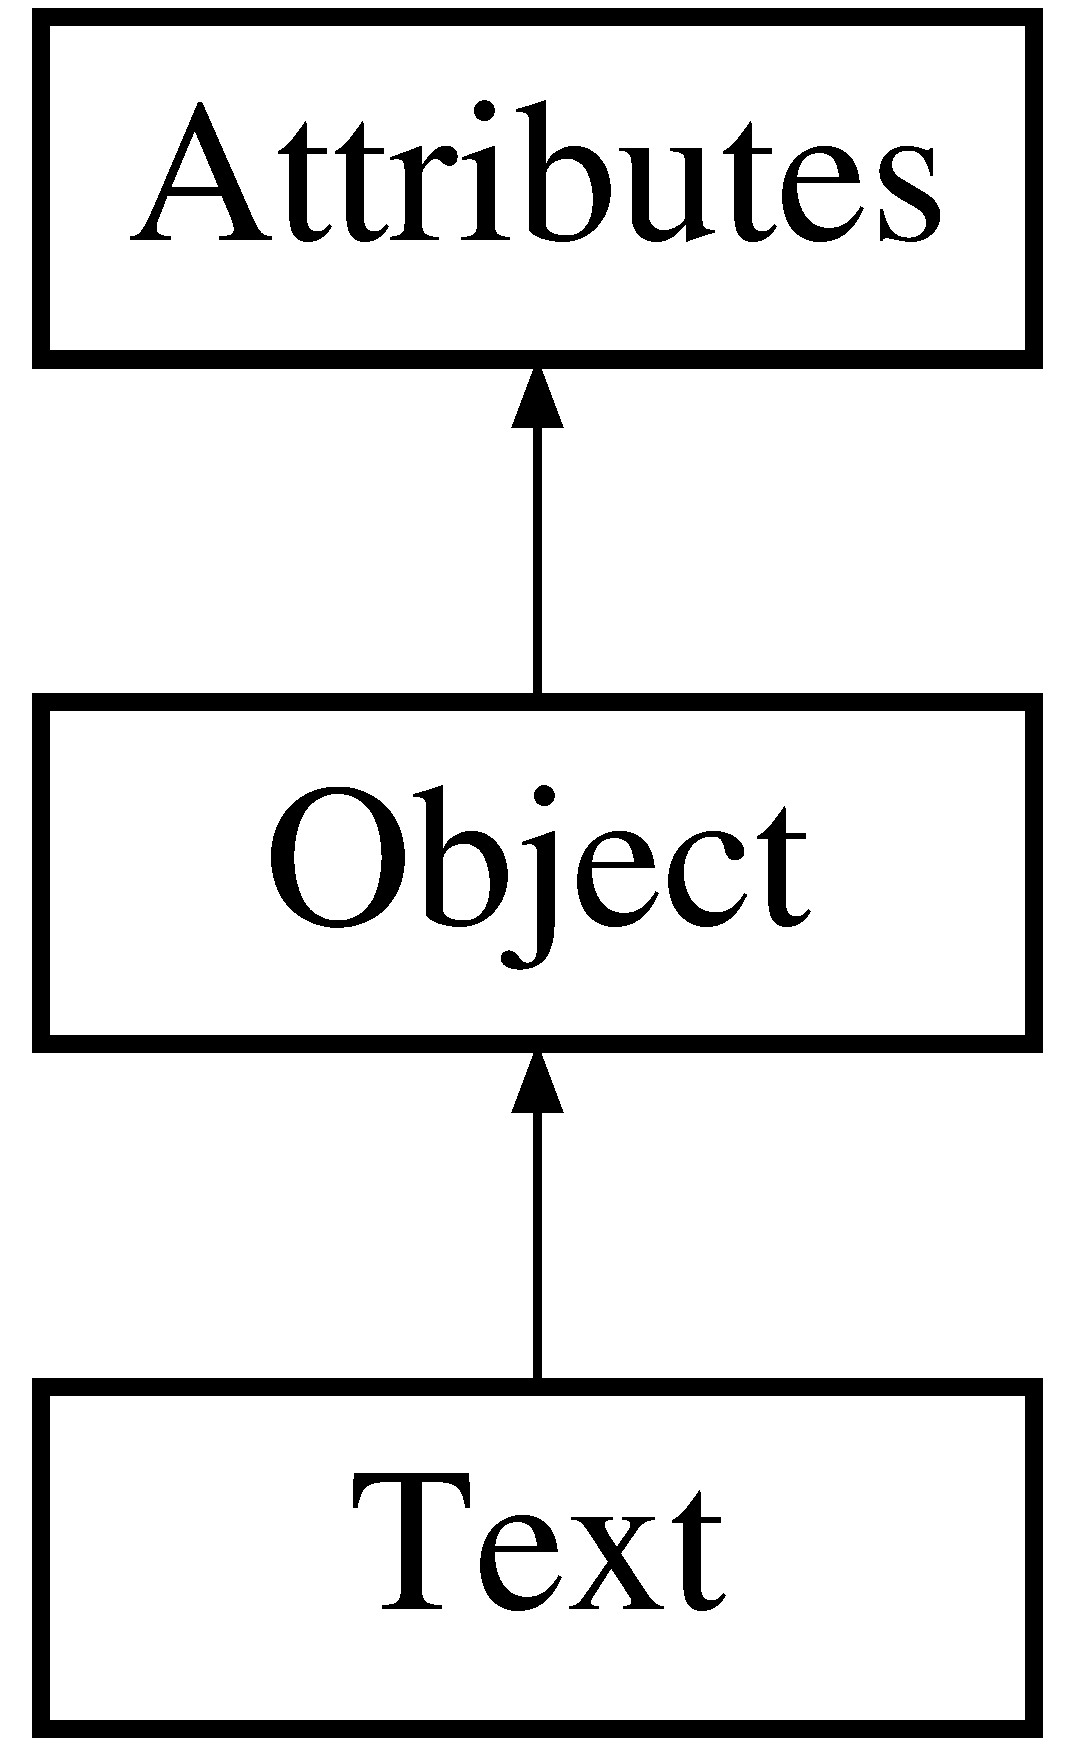
\includegraphics[height=3cm]{classText}
\end{center}
\end{figure}
\subsection*{Public Types}
\begin{CompactItemize}
\item 
enum {\bf Text\-Justifications} \{ {\bf Left\-Justified} =  0, 
{\bf Center\-Justified} =  1, 
{\bf Right\-Justified} =  2
 \}
\end{CompactItemize}
\subsection*{Public Methods}
\begin{CompactItemize}
\item 
{\bf Text} ()
\item 
{\bf Text} ({\bf Coordinate} $\ast${\bf place}, std::string {\bf contents})
\item 
{\bf $\sim$Text} ()
\item 
void {\bf set\-Justification} ({\bf Text\-Justifications} {\bf justification})
\item 
{\bf Text\-Justifications} {\bf get\-Justification} ()
\item 
void {\bf write} (std::ostream \&stream) const
\end{CompactItemize}
\subsection*{Protected Attributes}
\begin{CompactItemize}
\item 
{\bf Text\-Justifications} {\bf justification}
\item 
{\bf Coordinate} $\ast$ {\bf place}
\item 
std::string {\bf contents}
\end{CompactItemize}


\subsection{Detailed Description}
This class handles text objects. This class is derived from {\bf Object} {\rm (p.\,\pageref{classObject})}. \begin{Desc}
\item[Author: ]\par
Anthony Liekens \end{Desc}




\subsection{Member Enumeration Documentation}
\index{Text@{Text}!TextJustifications@{TextJustifications}}
\index{TextJustifications@{TextJustifications}!Text@{Text}}
\subsubsection{\setlength{\rightskip}{0pt plus 5cm}enum Text::Text\-Justifications}\label{classText_s3}


Enumeration of text justifications. The following justifications can be used to set the justification of a text object : \{$\backslash$tt Left\-Justified, Center\-Justified, Right\-Justified\} \begin{Desc}
\item[Enumeration values: ]\par
\begin{description}
\index{LeftJustified@{LeftJustified}!Text@{Text}}\index{Text@{Text}!LeftJustified@{LeftJustified}}\item[{\em 
{\em Left\-Justified}\label{classText_s3s0}
}]\index{CenterJustified@{CenterJustified}!Text@{Text}}\index{Text@{Text}!CenterJustified@{CenterJustified}}\item[{\em 
{\em Center\-Justified}\label{classText_s3s1}
}]\index{RightJustified@{RightJustified}!Text@{Text}}\index{Text@{Text}!RightJustified@{RightJustified}}\item[{\em 
{\em Right\-Justified}\label{classText_s3s2}
}]\end{description}
\end{Desc}



\subsection{Constructor \& Destructor Documentation}
\index{Text@{Text}!Text@{Text}}
\index{Text@{Text}!Text@{Text}}
\subsubsection{\setlength{\rightskip}{0pt plus 5cm}Text::Text ()}\label{classText_a0}


Constructor. Constructs a text object \index{Text@{Text}!Text@{Text}}
\index{Text@{Text}!Text@{Text}}
\subsubsection{\setlength{\rightskip}{0pt plus 5cm}Text::Text ({\bf Coordinate} $\ast$ {\em place}, std::string {\em contents})}\label{classText_a1}


Constructor. Constructs a text object \begin{Desc}
\item[Parameters: ]\par
\begin{description}
\item[{\em 
place}]- Instance of {\bf Coordinate} {\rm (p.\,\pageref{classCoordinate})}. Coordinates where the text object will be placed. \item[{\em 
contents}]- string \end{description}
\end{Desc}
\index{Text@{Text}!~Text@{$\sim$Text}}
\index{~Text@{$\sim$Text}!Text@{Text}}
\subsubsection{\setlength{\rightskip}{0pt plus 5cm}Text::$\sim$Text ()}\label{classText_a2}




\subsection{Member Function Documentation}
\index{Text@{Text}!getJustification@{getJustification}}
\index{getJustification@{getJustification}!Text@{Text}}
\subsubsection{\setlength{\rightskip}{0pt plus 5cm}{\bf Text\-Justifications} Text::get\-Justification ()\hspace{0.3cm}{\tt  [inline]}}\label{classText_a4}


Returns the text justification \begin{Desc}
\item[Returns: ]\par
Instance of {\bf Text\-Justifications} {\rm (p.\,\pageref{classText_s3})} \end{Desc}
\index{Text@{Text}!setJustification@{setJustification}}
\index{setJustification@{setJustification}!Text@{Text}}
\subsubsection{\setlength{\rightskip}{0pt plus 5cm}void Text::set\-Justification ({\bf Text\-Justifications} {\em justification})\hspace{0.3cm}{\tt  [inline]}}\label{classText_a3}


Set the text justification \begin{Desc}
\item[Parameters: ]\par
\begin{description}
\item[{\em 
justification}]{\bf Text\-Justifications} {\rm (p.\,\pageref{classText_s3})} \end{description}
\end{Desc}
\begin{Desc}
\item[Returns: ]\par
void \end{Desc}
\index{Text@{Text}!write@{write}}
\index{write@{write}!Text@{Text}}
\subsubsection{\setlength{\rightskip}{0pt plus 5cm}void Text::write (std::ostream \& {\em stream}) const\hspace{0.3cm}{\tt  [virtual]}}\label{classText_a5}


Write the text object to a given outstream. \begin{Desc}
\item[Parameters: ]\par
\begin{description}
\item[{\em 
stream}]output stream \end{description}
\end{Desc}
\begin{Desc}
\item[Returns: ]\par
void \end{Desc}


Reimplemented from {\bf Object} {\rm (p.\,\pageref{classObject_a3})}.

\subsection{Member Data Documentation}
\index{Text@{Text}!contents@{contents}}
\index{contents@{contents}!Text@{Text}}
\subsubsection{\setlength{\rightskip}{0pt plus 5cm}std::string Text::contents\hspace{0.3cm}{\tt  [protected]}}\label{classText_n2}


\index{Text@{Text}!justification@{justification}}
\index{justification@{justification}!Text@{Text}}
\subsubsection{\setlength{\rightskip}{0pt plus 5cm}{\bf Text\-Justifications} Text::justification\hspace{0.3cm}{\tt  [protected]}}\label{classText_n0}


\index{Text@{Text}!place@{place}}
\index{place@{place}!Text@{Text}}
\subsubsection{\setlength{\rightskip}{0pt plus 5cm}{\bf Coordinate}$\ast$ Text::place\hspace{0.3cm}{\tt  [protected]}}\label{classText_n1}




The documentation for this class was generated from the following files:\begin{CompactItemize}
\item 
{\bf text.h}\item 
{\bf text.cpp}\end{CompactItemize}
